\documentclass[a4paper,12pt]{article}
%\documentclass[doc]{apa}
\usepackage[usenames,dvipsnames]{color}
\usepackage{graphicx}
\usepackage{multicol}
\usepackage{multirow}
\usepackage{amsmath}
\usepackage{hyperref}
\usepackage{pdfpages}

%\setlength\parindent{0pt}
%\usepackage{figure}
\usepackage[margin=0.8in]{geometry}
\title{Project 1 Content Based Image Retrieval Using Global and Local Features}
\author{Daniel Bryan and Olmo Zavala\\Florida State University}

\begin{document}
\maketitle

For this project three approaches for Content Based Image Retrieval  (CBIR)
where implemented. The first approach is based on the comparison of color 
histograms, the second solution uses spectral histogram to do the comparison
of images, and the third approach uses SIFT features to compare images. 

\section{Description}
In this section the three methods used for CBIR are described. 

\subsection{Color histogram}
\label{sec_colorhist}
In this method we used the color (intensity filter) histogram  to 
compare images. The following steps summarizes the method:
\begin{enumerate}
    \item \textbf{Image pyramidization. } The images sizes where reduced
        to half in order to reduce the time of the algorithm. The method used
        to compute the pyramids is \emph{Gaussian pyramid}. The first
        step of the Gaussian pyramid algorithm is to blur the image 
        using a Gaussian filter, and then scale the image down by 
        creating one pixel from the average color of four pixels.
    \item \textbf{Compute histograms.} The number of bins used
        for this method is 256, for each color band.
    \item \textbf{Compute histogram distances.} The distance between
        each pair of image histograms was computed using histogram intersection:
        \begin{equation}
            dist(hist_a,hist_b) = \sum_{i=1}^{256} \min( hist_a(i), hist_b(i))
        \end{equation}
    \item \textbf{Images similarity}. The distance between the histograms
        of the images was used as the \emph{similarity} parameter. 
\end{enumerate}

\subsection{Spectral histogram}
\label{sec_spechist}
This method uses spectral histograms for CBIR. The proposed steps
for this method are as follows:

\begin{enumerate}
    \item \textbf{Image pyramidization. } The images sizes where reduced
        to half in order to reduce the time of the algorithm. The method used
        to compute the pyramids is \emph{Gaussian pyramid}. The first
        step of the Gaussian pyramid algorithm is to blur the image 
        using a Gaussian filter, and then scale the image down by 
        creating one pixel from the average color of four pixels.
    \item \textbf{Filter images}. Six filters in addition to the intensity
        filter are applied to each of the images. The filters 
        used and their corresponding masks are:
        \begin{equation}
            \begin{split}
                \frac{\partial I}{\partial x} & =  [0~-1~1] \\
                \frac{\partial I}{\partial y} & =  [0~-1~1]^T \\
                \frac{\partial I}{\partial x \partial x} & = [-1~2~-1] \\
                \frac{\partial I}{\partial y \partial y} & = [-1~2~-1]^T \\
                LoG(I(x,y))  & = ( x^2 + y^2 - \sqrt{2\sigma^2} ) e^{ -(x^2+y^2)/\sqrt{2\sigma^2}}\\
                Gauss(I(x,y))  & = \frac{1}{2 \pi \sigma^2} e^{ \frac{-(x.^2+y.^2)}{2\sigma^2}}\\
            \end{split}
        \end{equation}
        For the Laplacian of Gaussian (LoG) and Gaussian filters the size of the filter
        used is $5$ with a sigma value of $0.7$.
    \item \textbf{Compute spectral histograms.} The number of bins used
        for this method is 100, for each color band and for each filter. 
        For all of the filters the range goes from [0 256], even when the values of some
        of the filters may go from [-256 256]. Several options for the range of the 
        histograms were tested, and the range of [0 256] gave the best results. 
        The 100 bins were evenly split from [0 256].
        Figure \ref{fig:spechist} shows an example of the spectral histograms. 
        \begin{figure}[h]
            \centering
            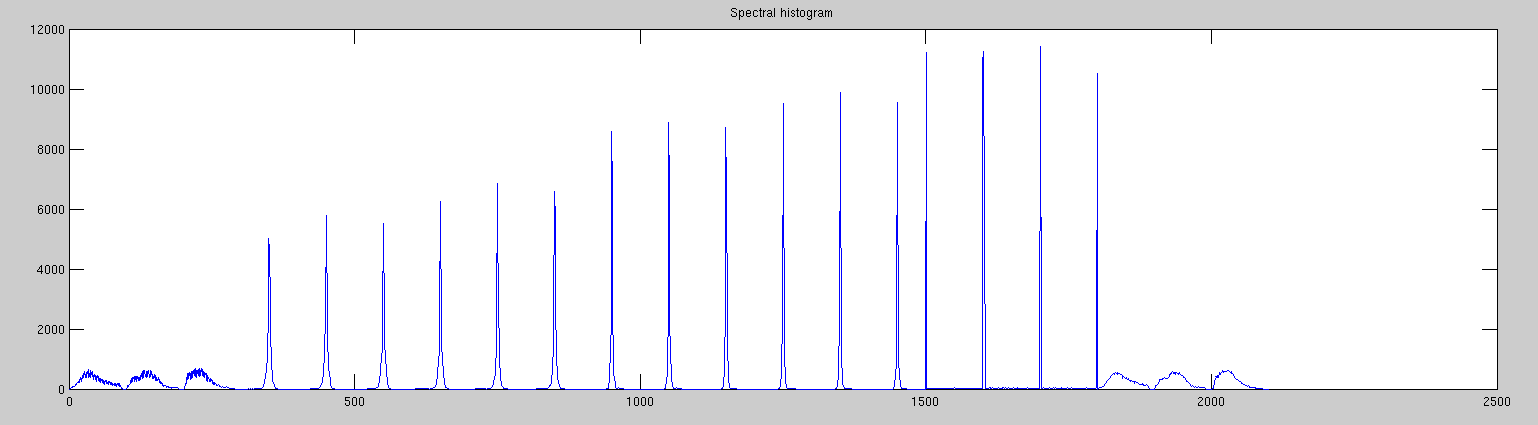
\includegraphics[totalheight=.18\textheight]{./Images/SpectralHist.png}
            \label{fig:spechist}
        \end{figure}
    \item \textbf{Compute histogram distances.} The distance between
        each pair of image histograms was computed using histogram intersection:
        \begin{equation}
            dist(hist_a,hist_b) = \sum_{i=1}^{100} \min( hist_a(i), hist_b(i))
        \end{equation}
    \item \textbf{Images similarity}. The distance between the histograms
        of the images was used as the \emph{similarity} parameter. 
\end{enumerate}

\subsection{Scale-Invariant Feature Transform (SIFT)}
For this method we used the SIFT descriptors to compare images. The code is based on  
the implementation provided at \href{http://www.vlfeat.org/}{http://www.vlfeat.org/}. The proposed steps
to obtain a score that could be used for CBIR are as follows:

\begin{enumerate}
    \item Obtain the SIFT descriptors for each image using function \textbf{vl\_sift}. 
    \item Compute the matching descriptors and the distance between those descriptors using
        the function \textbf{vl\_ubcmatch}.
    \item Obtain the maximum distance obtained between all the matches (for later normalization).
    \item Combine the average distance of the matched descriptors with the 
        number of matched descriptors between two images using \emph{Cantor pairing}. Equation \ref{eq:sift}
        shows the score computed between images $i$ and $j$ using the SIFT features.
        \begin{equation}
            \begin{split}
                k1 & = mean( \frac{\text{matches}(i,j)}{\text{maxDist}})\\
                k2 & = \text{length}(\text{matches}(i,j))\\
                \text{siftScore}(i,j) & =  (0.5*(k1+k2)*(k1+k2+1))+k2
            \end{split}
            \label{eq:sift}
        \end{equation}
\end{enumerate}


\subsection{Computation time}
The three methods were implemented in parallel (when possible) using the
matlab function $parfor$. The third method, which uses SIFT features,
takes significantly more time and is presented separately at the end of this section. \\

For efficiency, the first two methods are implemented in the same code, but the program 
\emph{Problem1And2CompTime} can be easily modified to display the time that
takes for each method to compute the CBIR. The times shown in table \ref{tab:times}
are for a specific run on a machine running Ubuntu 14.04, with matlab 2012a, 
with an i7 intel processor and 10 GB of ram. The times varies a little for each run
but table \ref{tab:times} gives a good approximation of the time that each method takes.
\begin{table}[h!]
    \centering
    \begin{tabular}{|c|c|c|}
        \hline
        & \textbf{Color Hist (sec)} & \textbf{Spectral Hist (sec)} \\
        \hline
        \text{Read images, filter } & & \\
        \text{and compute histogram} & 9.38 & 30.01 \\
        \hline
        \text{Calculate distances} & 6.69 & 10.78  \\
        \hline
        \text{Compute Precision Recall } & 1.47 & 1.45 \\
        \hline
        \text{Avg. Precision and Rank} & 1.22 & 1.34 \\
        \hline
        \textbf{Total time} & \textbf{17.54} & \textbf{43.58}\\
        \hline
    \end{tabular}
    \label{tab:times}
\end{table}

The method based on SIFT features takes significantly more time to complete. In order to 
debug our proposed method, the computation of the SIFT features and descriptors was run once
and then saved in a separate file (\emph{/Variables/descriptors.mat}). The results of the descriptor matching, which takes almost two hours to finish,
were also saved in a separate file (\emph{/Variables/scores.mat}). In this way
we only had two compute the matching and the descriptors once for the image set. The times shown
in table \ref{tab:sift} are also obtained from a Laptop computer running Ubuntu 14.04, with matlab 2012a, 
with i7 intel processor and 10 GB of ram. 
\begin{table}[h!]
    \centering
    \begin{tabular}{|c|c|}
        \hline
        & SIFT (time sec) \\
        \hline
        \text{Read all Images} & 12.47 \\
        \hline
        \text{Detect SIFT descriptors} & 83.3 \\
        \hline
        \text{Matching descriptors} & approx. 7 sec/image\\
        & $\sim$ 7000 sec $\sim$ 1:56 hrs\\
        \hline
        \text{SIFT score} & 18.8 \\
        \hline
        \text{Precision recall} & 1.6 \\
        \hline
        \text{Average PR} & 1.44 \\
        \hline
        \textbf{Total} & $\sim$ \textbf{2 hrs}\\
        \hline
    \end{tabular}
    \label{tab:sift}
\end{table}

\section{Results}

To better compare the results between the proposed methods, the results were plotted together. Figure \ref{fig:res} displays the average precision (left) and average rank (right) for each of the ten classes of images. There are four methods analyzed: SIMPLIcity (red star),
color histogram (green circle), spectral histogram (blue square), and SIFT features (magenta diamond).\\

The highest performing of the proposed methods is the \textbf{Spectral Histogram}. It improves the results shown in 
the SIMPLIcity paper in 8 of the 10 categories for the average precision and in 2 
of the 10 categories for the average rank. The \textbf{Color histogram} method obtained
higher average precision for some of the categories (1, 8, and 10), but in general is 
a little bit behind than the Spectral histogram method. The \textbf{SIFT} features 
method seems to over fit the matching of the images and in general obtained poor results. 
This method is still the only one that surpasses SIMPLIcity for the 3rd category in the average precision
evaluation. We believe that the problem of the method used compare images based on the
SIFT features is that it is not taking into account a 'general' similarity between the descriptors. 
The function that was used (vl\_ubmatch) computes the closest descriptors and their distances, but there is no indication that images in the same class consistently share similar features. A better approach may 
be to match only the most representative features between the images, which may require semantic interpretation. 

\begin{figure}[h!]
    \centering
    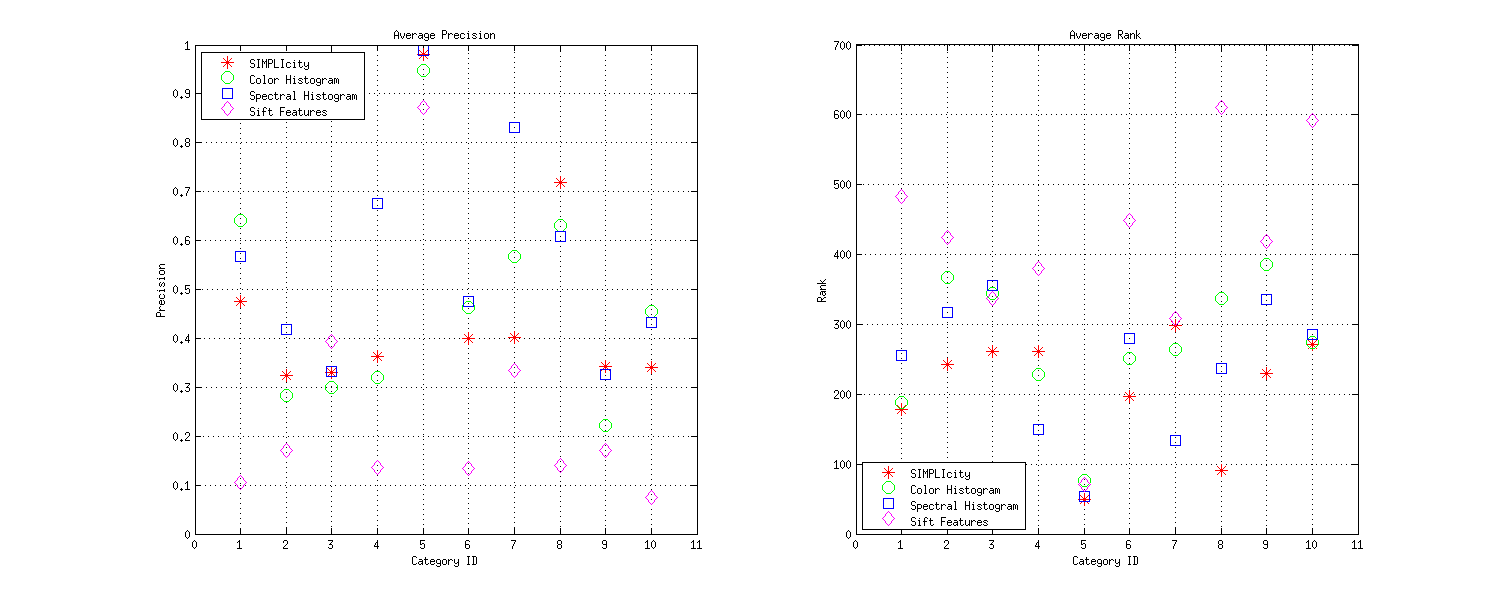
\includegraphics[totalheight=.26\textheight]{./Images/AllResults.png}
    \label{fig:res}
\end{figure}

The following are good and bad examples of Precision/Recall curves (PR) obtained for each methods. Figure \ref{fig:good} shows the PR obtained for image $\#401$ using 
color histogram and spectral histogram methods. In this case both methods obtained good PR curves. 

\begin{figure}[h!]
    \centering
    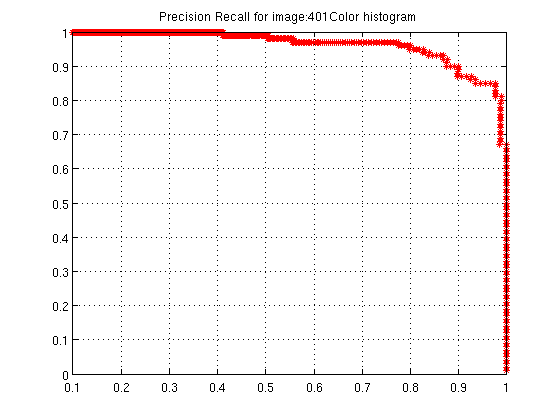
\includegraphics[totalheight=.24\textheight]{../Results/PR/GoodColor.png}
    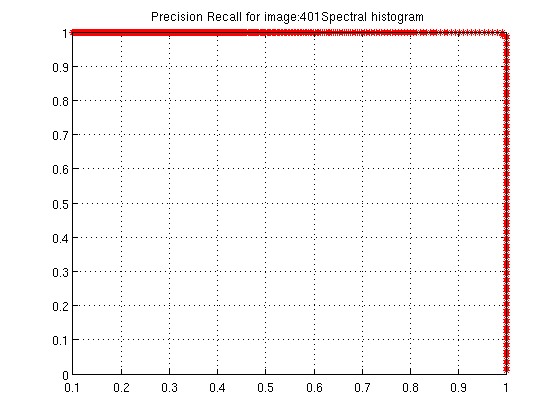
\includegraphics[totalheight=.24\textheight]{../Results/PR/GoodSpectral.png}
    \label{fig:good}
\end{figure}

Figure \ref{fig:bad} shows the PR obtained for image $\#361$ color histogram and spectral histogram methods. In this case both methods obtained poor PR curves.
\begin{figure}[h!]
    \centering
    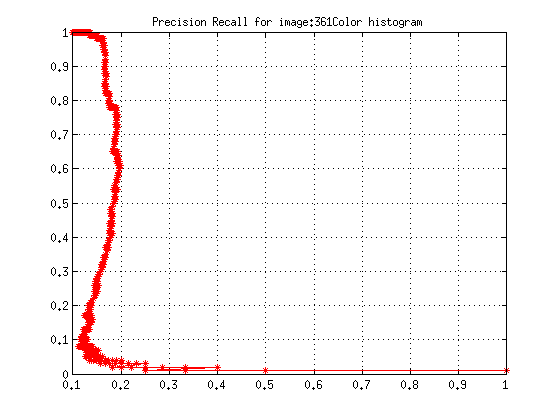
\includegraphics[totalheight=.24\textheight]{../Results/PR/BadColor.png}
    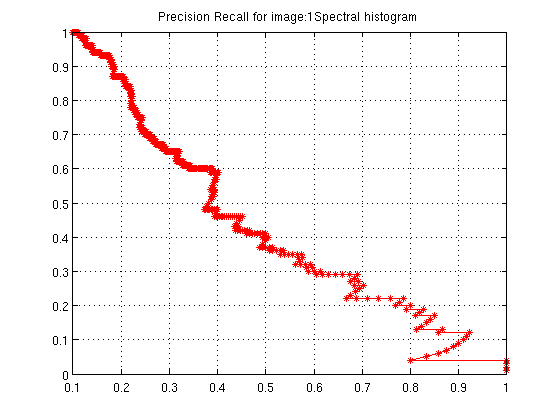
\includegraphics[totalheight=.24\textheight]{../Results/PR/BadSpectral.png}
    \label{fig:bad}
\end{figure}

Finally, figure \ref{fig:sgb} shows the PR curves obtained using the SIFT features method.
The first case is the image $\#481$ which obtains very good results. 
The right plot of figure \ref{fig:sgb} shows the PR curve for image $\#331$ where it obtains very poor results.
\begin{figure}[h!]
    \centering
    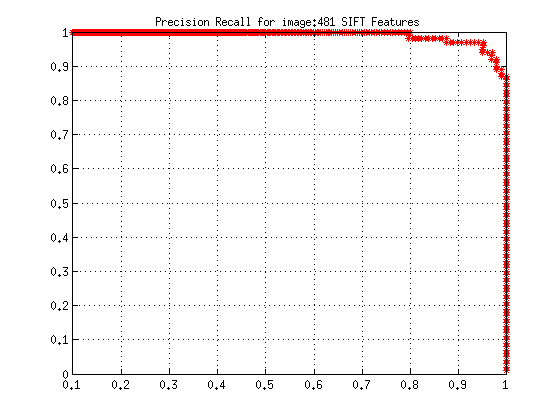
\includegraphics[totalheight=.24\textheight]{../Results/PR/GoodSIFT.png}
    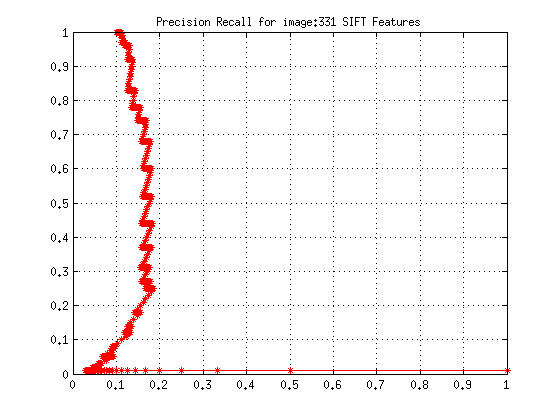
\includegraphics[totalheight=.24\textheight]{../Results/PR/BadSIFT.png}
    \label{fig:sgb}
\end{figure}

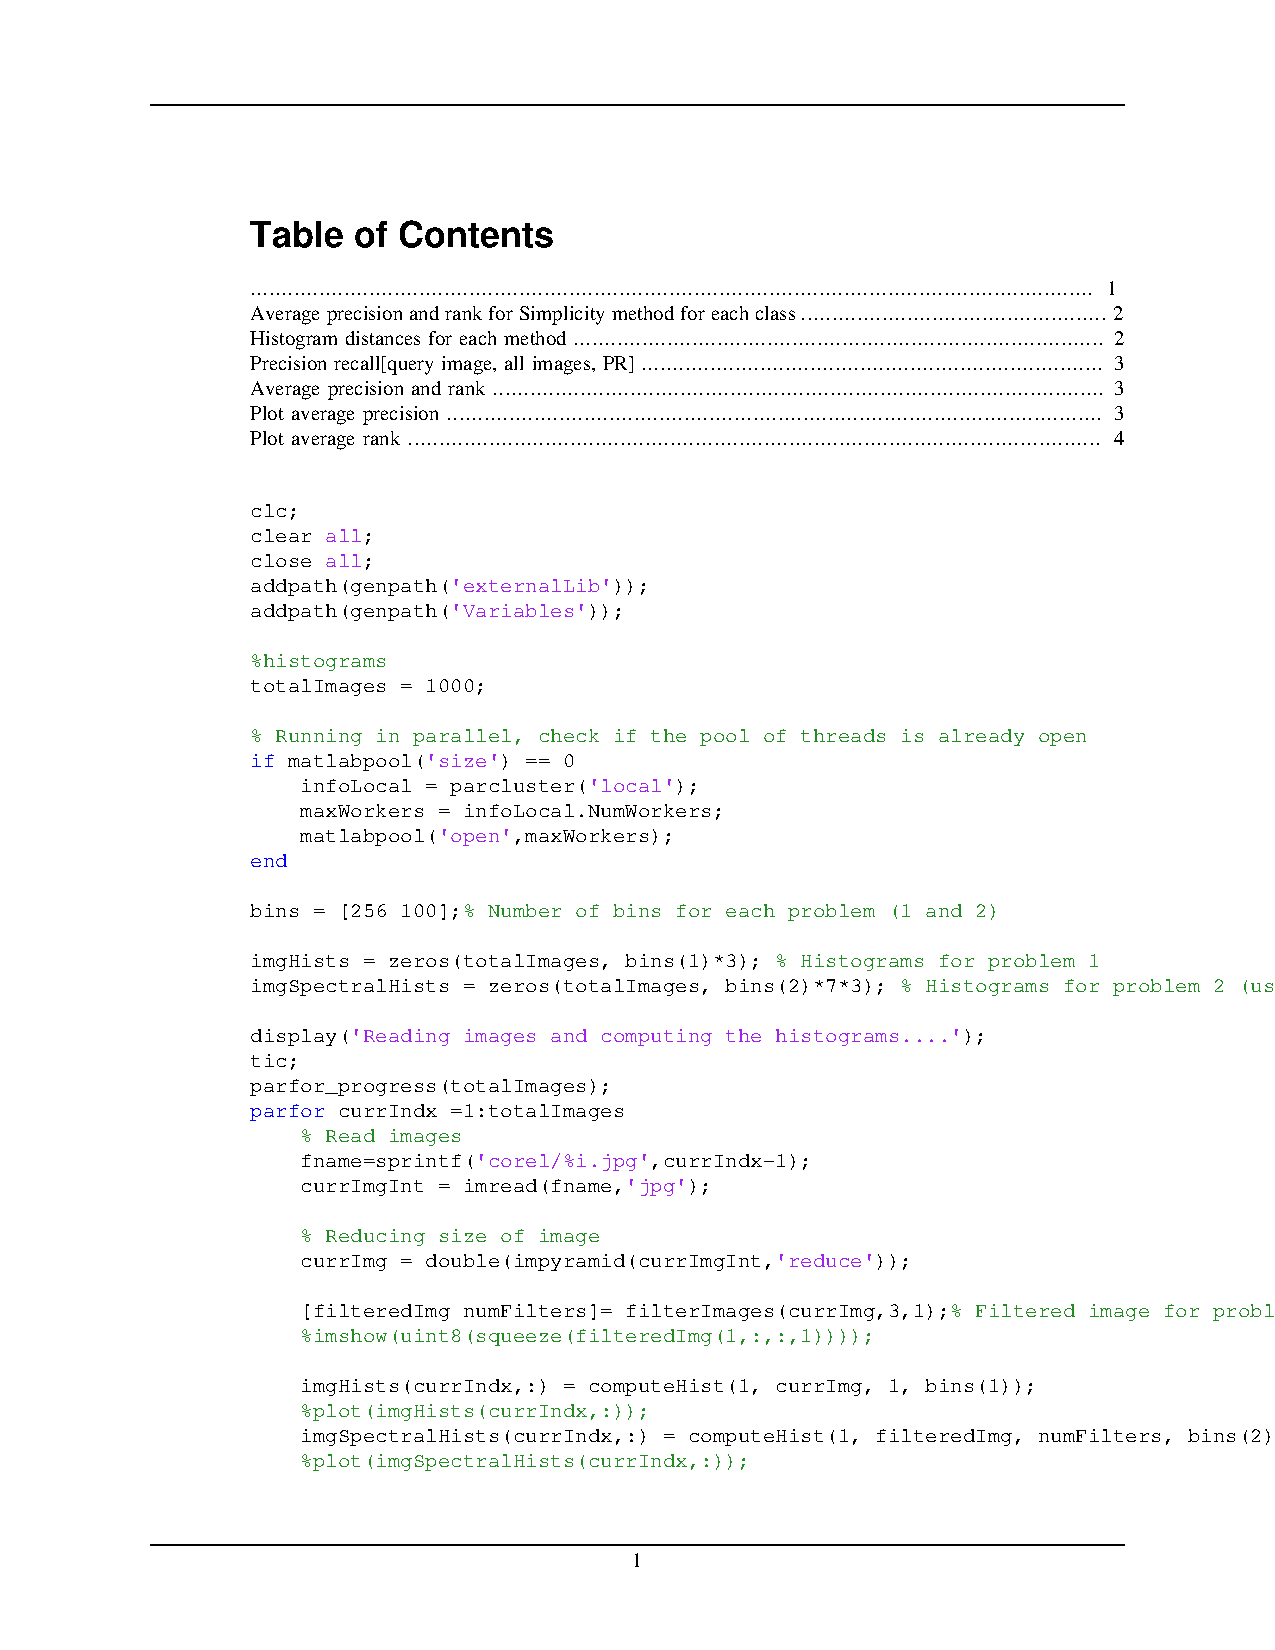
\includepdf[pages={1-15}]{FromMatlab/Code.pdf}

\end{document}
